\section{Analyse}
Vi har indelt problemet i forskellige concepter, der hver har deres eget ansvar, resultatet kan ses herunder.
\begin{figure}
  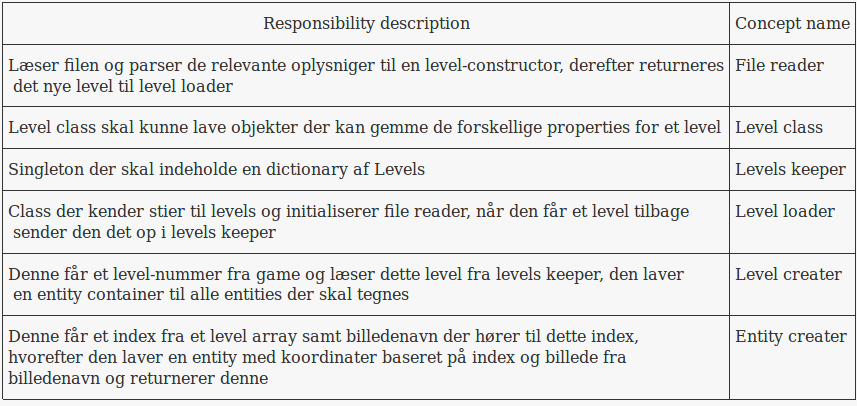
\includegraphics[width=15cm]{latex/ResponsibilityDescription}
  \caption{Koncepter og deres ansvar}
\end{figure}
Vi har opdelt koncepterne efter koncepttyperne Know og Do, så hvert koncept har netop én type. Vores Do koncepter har hver ansvar for én opgave, eksempelvis file reader der kun skal lave et level ud fra informationen fra en fil. Vi har 6 koncepter hvoraf 4 er Do- og 2 er know-koncepter.\\
Vores entity creator laver for nu kun firkanter der alle er lige store, og som har et billede, da vi antager vi ikke skal implementere collision detection i denne uge. På længere sigt skal der være forskel på størrelsen og formen på de forskellige objeker.

\begin{figure}
  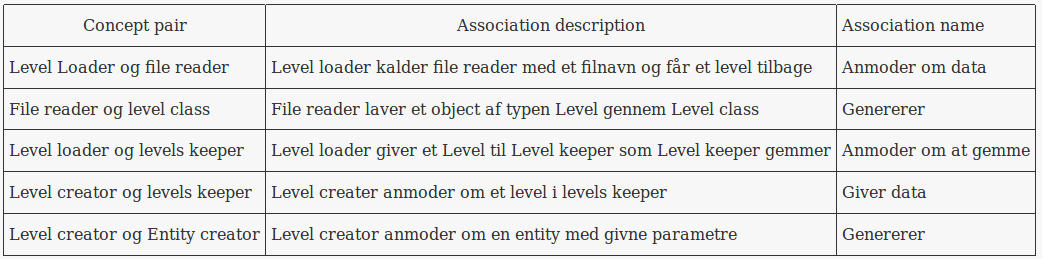
\includegraphics[width=15cm]{latex/ConceptPairs}
  \caption{Associationer mellem concepter}
\end{figure}

\begin{table}[]
\centering
\caption{My caption}
\label{my-label}
\begin{tabular}{|l|l|l|}
\hline
Concept                      & Attribute        & Attribute description                                                                 \\ \hline
Level loader                 & Levels           & En liste af filnavnene på level layouts                                               \\ \hline
File reader                  & Ingen attributer &                                                                                       \\ \hline
\multirow{5}{*}{Level class} & Level array      & 2D-struktur der indeholder level design                                               \\ \cline{2-3}
                             & Name             & Navn på level                                                                         \\ \cline{2-3}
                             & Costommer        & Information om costommers i dette level                                               \\ \cline{2-3}
                             & Platforms        & Liste med information om hvilke dele af level layout der svarer til platforme I level \\ \cline{2-3}
                             & Decoder          & Denne gemmer sammenhængen mellem karakterer og billedenavne                           \\ \hline
Levels keeper                & Levels           & Contatiner til alle levels                                                            \\ \hline
                             & Index            & Tæller der holder styr på hvor mange levels der er I levels                           \\ \hline
Level creator                & Levels           & Reference levels keepers                                                              \\ \hline
Entity creator               & Ingen attributer &                                                                                       \\ \hline
\end{tabular}
\end{table}
